\subsection{Dataset}
We have conducted experiments on the following datasets(Mainly For Phase 1):
\begin{center}
\begin{tabular}{| l | c |}
  \hline                        
  Dataset Name & Advogato  \\ \hline
  Largest conn compo & 5054  \\ \hline
  Size & 6551 vertices  \\ \hline
  Volume & 51332 edges \\ \hline
\end{tabular}
\end{center}

In out final experiment suit, a more large and diverse datasets from different domains will be explored. The tentative source of experiment dataset are listed below:
\begin{description}
	\item{{\bf SNAP:}}{It has abundant data about social network, we plan to conduct triangle counting, pagerank, radius computing experiment which will reveal the underlying feature of large graphs and spot strange graphs.}
	\item{{\bf Konect:}}{Konect has more diverse datasets compared to SNAP, like citation network. It's a good target to analyze features of non-social networks, we will examine whether such networks follow power law by generating degree distribution, etc.}
\end{description}

In phase 1, we explored Task 1-3, and do several visualization for experiment results. Figure \ref{fig:results}(a) shows the in degree distribution, we took log of rank to emphasize the effect. Figure \ref{fig:results}(b) shows the out degree distribution, also took logarithm. Figure \ref{fig:pagerank} plots the distribution of different rank value.We also calculated statistics about the weakly connected components in table \ref{table:wcc}.We compute radius for every node in Advogato dataset, the result is in table \ref{table:radius}:

\begin{figure}[htbf]
\begin{center}
\begin{tabular}{cc}
     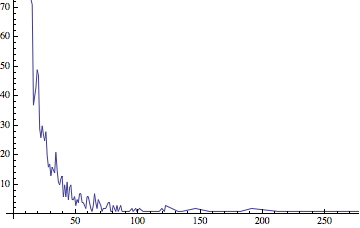
\includegraphics[width=0.4\textwidth]{FIG/indegree.png} &
     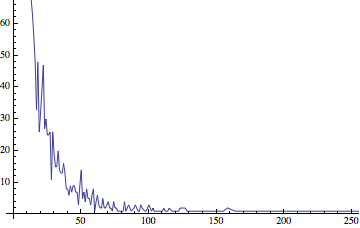
\includegraphics[width=0.4\textwidth]{FIG/outdegree.png} \\
    (a) & (b) 
\end{tabular}
\caption{In degree distribution (a) and out degree distribution (b)}
\label{fig:results}
\end{center}
\end{figure}

\begin{figure}[htbf]
\begin{center}
     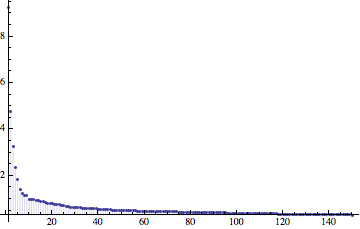
\includegraphics[width=0.6\textwidth]{FIG/pagerank.png}
\caption{Pagerank distribution}
\label{fig:pagerank}
\end{center}
\end{figure}


\begin{table}
\begin{center}
\begin{tabular}{| l | c |}
  \hline                        
  Size of WCC & Count  \\ \hline
  1 & 1384  \\ \hline
  2 & 55  \\ \hline
  3 & 1 \\ \hline
  5054 & 1 \\ \hline  
\end{tabular}
\caption{Statistics about Weakly connected components}
\label{table:wcc}
\end{center}
\end{table}

\begin{table}
\begin{center}
\begin{tabular}{| l | c |}
  \hline                        
  radius & number of vertices  \\ \hline
  0 & 1896  \\ \hline
  1 & 84  \\ \hline
  2 & 11 \\ \hline
  3 & 7 \\ \hline  
  4 & 634 \\ \hline  
  5 & 2194 \\ \hline  
  6 & 826 \\ \hline  
  7 & 117 \\ \hline  
  8 & 13 \\ \hline
  9 & 2 \\ \hline   
\end{tabular}
\caption{statistics about radius}
\label{table:radius}
\end{center} 
\end{table}

\begin{figure}[htbf]
\begin{center}
     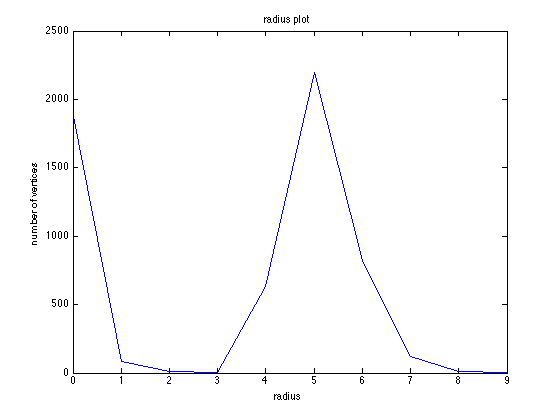
\includegraphics[width=0.6\textwidth]{FIG/radius.png}
\caption{Radius Plot}
\label{fig:radius}
\end{center}
\end{figure}

\subsection{Triangle Counting(Design)}
The main reason of triangle counting is to compare the capability of each solution(RDBMS, general purpose programming language). We will apply RDBMS version and c++/java version, record their running time and resource usage, then do performance analysis. 

\subsection{Belief Propagation(Design)}
In order to investigate the gain of using RDBMS, We plan to compare the efficiency of RDBMS's implementation of BP with BP in general purpose languages like c++/java. We ponder that the difference will be only observable in large dataset, we will conduct experiments to try to estimate that. 

\subsection{Eigenvalue/SVD(Design)}
SVD is a powerful tool at dimension reduction, or in another words, clustering. So We plan to apply SVD to social networks to find communities, and some work has been done by researchers in data mining and matrix analysis. 

